% >8----------------------------ESTRUTURAS DE DADOS EM SCHEME----------------------------8<
\section{Pares}
\begin{frame}
  \frametitle{Estruturas de Dados a partir de pares}
  \only<1>{
    \begin{center}
      \textit{Pairs provide a universal building block from which \\
                we can construct all sorts of data structures.}\\
          --- Harold Abelson e Gerald Jay Sussman
    \end{center}
  }
  \only<2>{
    \begin{figure}
      \centering
      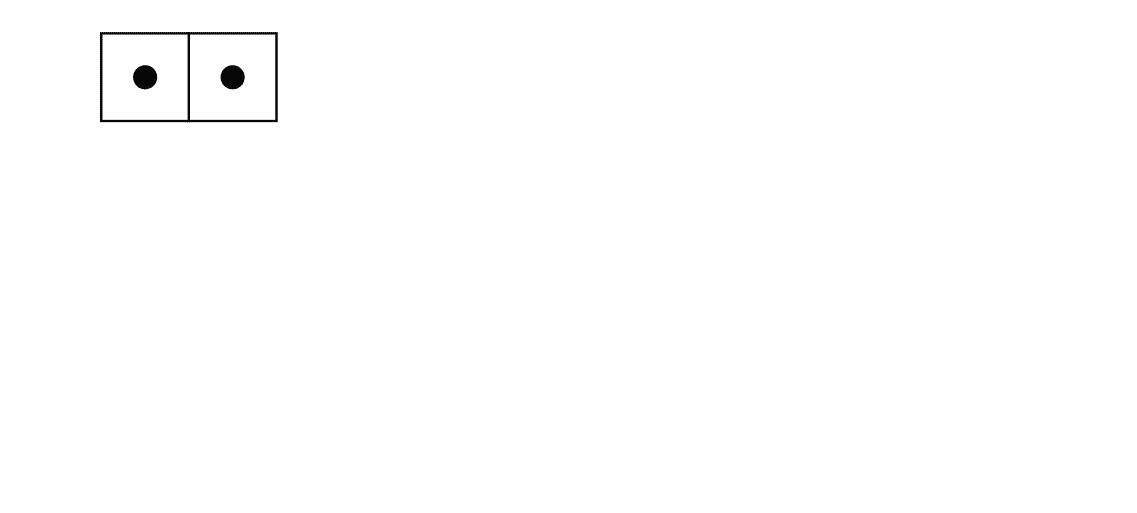
\includegraphics[width=0.7\linewidth]{pairs-1.png}
    \end{figure}
  }
  \only<3>{
    \begin{figure}
      \centering
      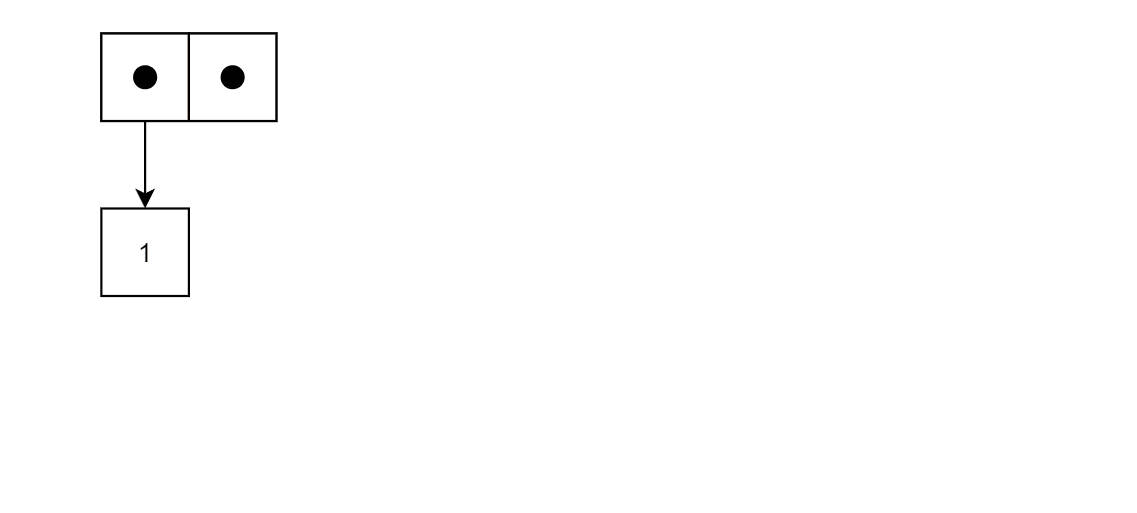
\includegraphics[width=0.7\linewidth]{pairs-2.png}
    \end{figure}
  }
  \only<4>{
    \begin{figure}
      \centering
      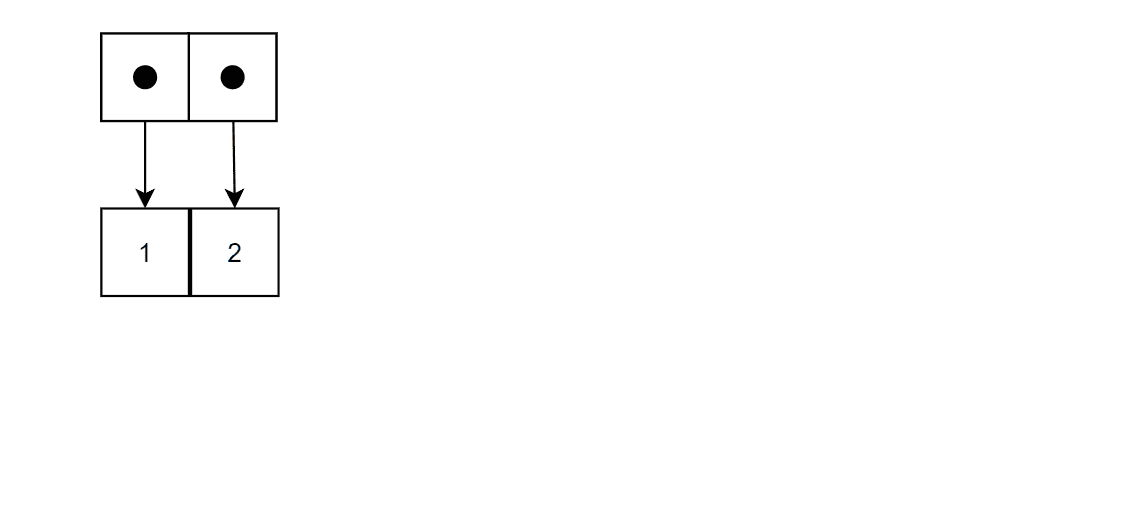
\includegraphics[width=0.7\linewidth]{pairs-3.png}
    \end{figure}
  }
  \only<5>{
    \begin{figure}
      \centering
      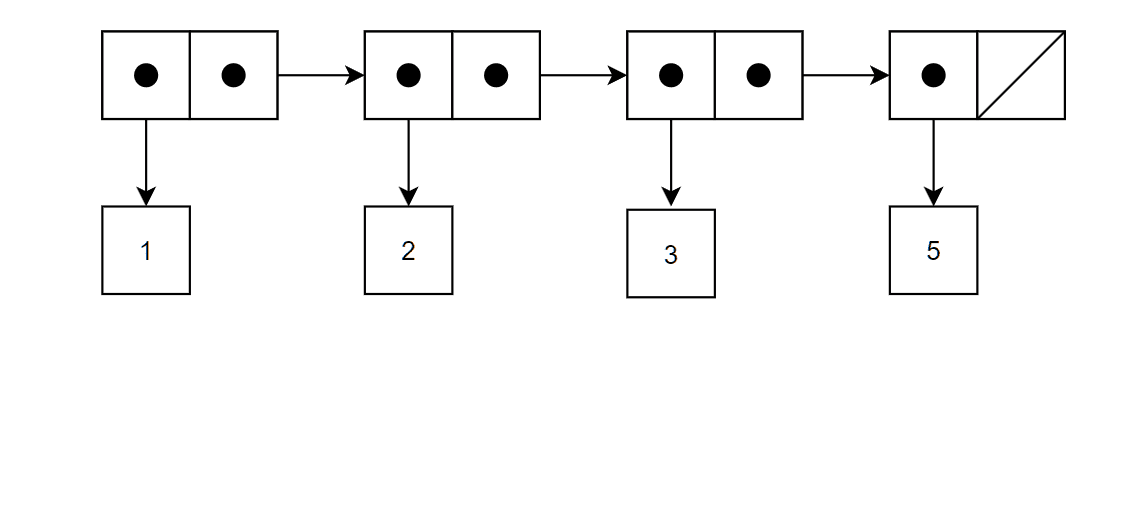
\includegraphics[width=0.7\linewidth]{pairs-4.png}
    \end{figure}
  }
  \only<6>{
    \begin{figure}
      \centering
      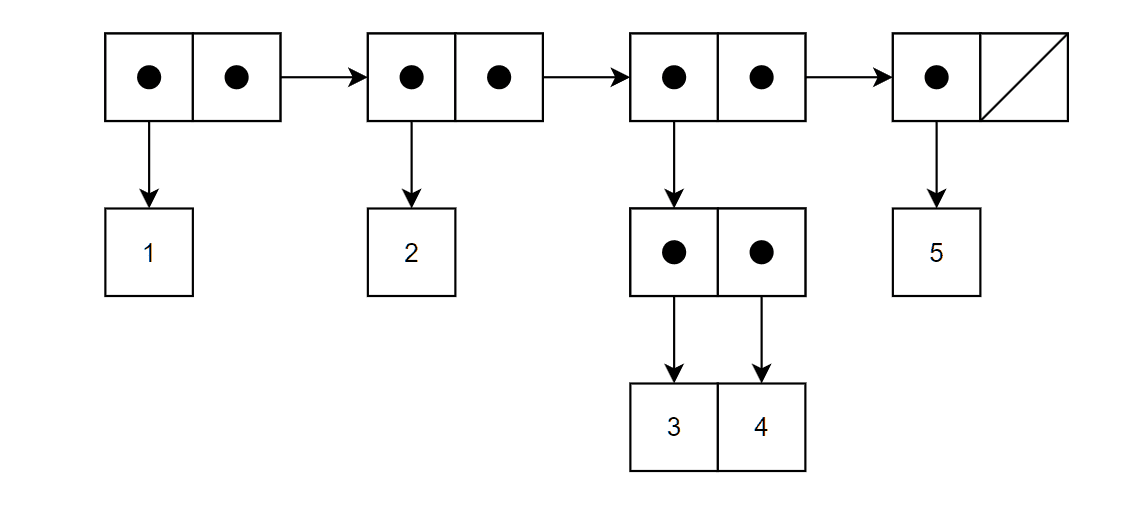
\includegraphics[width=0.7\linewidth]{pairs-5.png}
    \end{figure}
  }
\end{frame}
% >8----------------------------ESTRUTURAS DE DADOS EM SCHEME----------------------------8<



% >8------------------------------------POR QUE PARES?-----------------------------------8<
\begin{frame}
  \frametitle{Representações: Pares}
  \framesubtitle{Por que Pares?}

  \begin{center}
  \textit{Once you have two things, you \\
            have as many things as you want.}\\
      --- Harold Abelson
  \end{center}
  \pause
  \vspace{0.5cm}
  Três simples procedimentos:

  \begin{itemize}
    \item \texttt{cons} \hspace{0.4cm} $\mid$ \hspace{0.4cm} \texttt{(cons x y)} $\mapsto$ \texttt{(x y)} \\
    \item \texttt{car } \hspace{0.4cm} $\mid$ \hspace{0.4cm} \texttt{(car (x y))} $\mapsto$ \texttt{x} \\
    \item \texttt{cdr } \hspace{0.4cm} $\mid$ \hspace{0.4cm} \texttt{(cdr (x y))} $\mapsto$ \texttt{y} \\
  \end{itemize}
\end{frame}
% >8------------------------------------POR QUE PARES?-----------------------------------8<



\begin{frame}[fragile]
  \begin{code}

>> (cons 1 2)
(1 2)
  \end{code}
  \pause
  \begin{code}

>> (cons 1 (cons 2 (cons 3 (cons 5 '()))))
(1 2 3 5)
  \end{code}
  \pause
  \begin{code}

>> (cons 1 (cons 2 (cons (cons 3 4) (cons 5 '()))))
(1 2 (3 4) 5)
  \end{code}
\end{frame}